\documentclass[12pt]{article}
%\usepackage{scicite}
\usepackage{times}
\usepackage{graphicx}

% The following parameters seem to provide a reasonable page setup.
\topmargin 0.0cm
\oddsidemargin 0.2cm
\textwidth 16cm 
\textheight 21cm
\footskip 1.0cm


%The next command sets up an environment for the abstract to your paper.
\newenvironment{sciabstract}{%
\begin{quote} \bf}
{\end{quote}}


\title{Motion Challenge: Hitting a Ball with a racket } 
\author{}
\date{}
%%%%%%%%%%%%%%%%% END OF PREAMBLE %%%%%%%%%%%%%%%%

\begin{document} 

\maketitle 

% Place your abstract within the special {sciabstract} environment.
\begin{sciabstract}
\end{sciabstract}


\section*{Basic challenge description}
The goal of the motion challenge is that the robot has to hit the ball with a racket in such a way that the ball flies as far as possible. The ball will be spawned at a specific position and flies in the direction to the robot. The robot should decide if he needs to use the backhand or the forehand depending on high the ball is in the air.

\begin{figure}[h]
	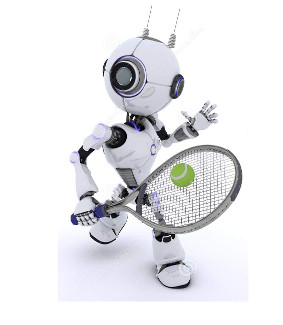
\includegraphics[scale=0.5]{backhand}
	\centering
	\caption{Example of hitting the ball with the backhand}
\end{figure}

\section*{Additional challenge description}
If you have an good solution for the challenge one improvement of the challenge will be to hit the ball in such a way that the ball will hit a specific target/object. 



\end{document}




















